\section{Test setups, data and reconstruction}\label{sec:setups}
\sectionstate{ready}{\texttt{mx\_june\_cosmic\_qa/MICROTPC\_RUNBOOK.md}; \texttt{sps\_beam\_test\_26/analysis/README.md}. v2 2026-11-10: the
beam setup drawing joins the bench drawing (\cref{fig:setups}); the run-by-run comparison of Runs 1 and 2 is one
sentence here and a figure in \cref{app:gain}; the terms used by every later section are defined once in \cref{sec:definitions}.}
\intent{The two setups and what each can measure, the chambers and runs, the reconstruction in one paragraph, and the
definitions every result uses.}

\subsection{Cosmic bench}
\tbw{Scintillator trigger, four reference tracking planes, two test slots. DREAM readout, sampling, window. Gas and flow.}
\askDylan{Gas per setup: bench Ar/iC$_4$H$_{10}$ 95/5? SPS runs with Ar/CF$_4$/iC$_4$H$_{10}$ 88/10/2? Which runs enter the paper?}
The bench (\crefp{fig:setups}{a}) triggers on the coincidence of two scintillators and carries four reference tracking
planes, two above and two below the chamber under test, over a lever arm of 1278\,mm. A track reconstructed in them
with one cluster per plane and $\chi^2<1.0$ is called the \emph{reference track}, and its extrapolation to the chamber
under test the \emph{reference ray}. At the chamber the reference ray points to 0.21--0.28\,mm per coordinate, and its
angle is known to better than 0.14\textdegree{} (\cref{sec:angle}).

\subsection{SPS H4 beam}
Only chamber~E went to the SPS: the test (late July -- early August 2026; exact dates to fill from the run log) ran while
chambers A--D were installed at n\_TOF, so the one chamber not needed there, with its known non-amplifying stripes
(\cref{app:beam}), was the one available. The beam crosses two uRWELL reference trackers and chamber~E, which could be
yawed by 25.4\textdegree{} (\crefp{fig:setups}{b}).
\tbw{Beam, runs used (HV, drift field, gas, rotation).}
The beam data are a cross-check in this paper. Every headline number comes from the cosmic bench. The beam confirms
the position resolution (\cref{sec:position}) and, at an angle the bench does not reach, the angle scale
(\cref{sec:angle}), and it shows the same gas analysis at work in other mixtures (\cref{sec:attachment}).
% NOTE (Dylan, 2026-11-09): mount angle 25.4 deg = measured yaw from the run-57 alignment (25.52 = midpoint of the measured
% yaw and the configuration value; 25.64 = run-configuration value det_orientation.y, the old "25.6").

\begin{figure}[tbp]
  \centering
  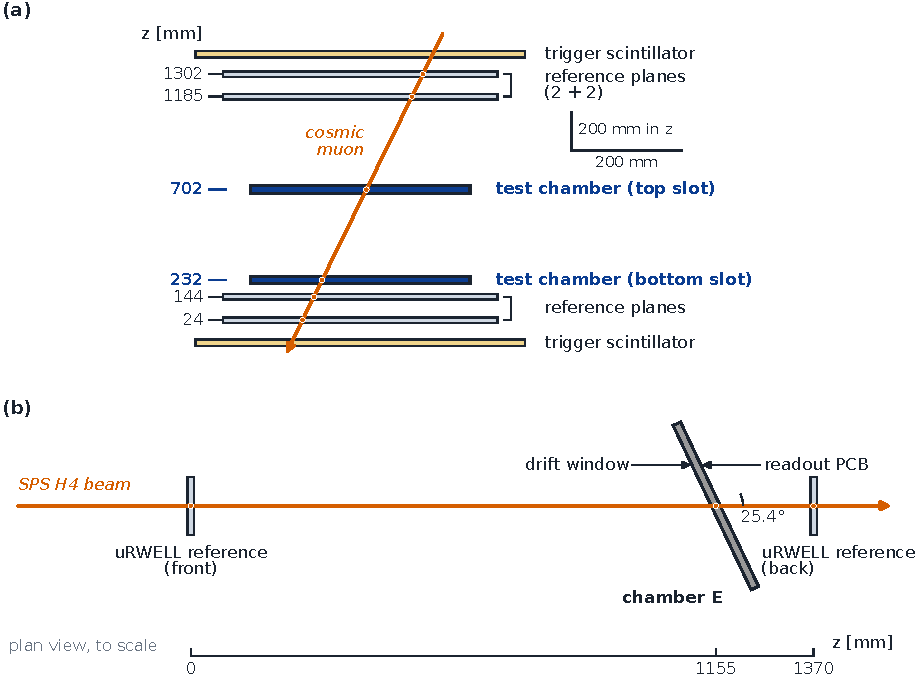
\includegraphics[width=0.86\linewidth]{setups}
  \caption{The two test setups. (a) The Saclay cosmic bench, side view, muons going down ($z$ drawn compressed to 0.35
  of the transverse scale, as the scale bars show; slab thicknesses exaggerated). The readout is triggered by the
  coincidence of the top and bottom scintillators ($60\times60$\,cm). The four reference planes ($50\times50$\,cm;
  $z=24$, 144, 1185, 1302\,mm) reconstruct each muon independently of the chamber under test. The two test slots are
  at $z=232$ and 702\,mm; chamber~A ran in the top slot for Runs 1 and 2. Scintillator positions are schematic.
  (b) The SPS H4 setup, plan view, to scale (slab thicknesses exaggerated): the beam crosses two uRWELL reference
  trackers ($z=0$ and 1370\,mm) and chamber~E, yawed by 25.4\textdegree{} about the vertical, so that beam tracks cross
  its drift gap at that angle. The drift window faces upstream.}
  \label{fig:setups}
\end{figure}

\subsection{Chambers and data sets}\label{sec:datasets}
% Public names (Dylan 2026-11-03). Internal keys, for the analysis code and logbooks:
%   A = det3 (mx17_3), B = det2 (mx17_2), C = det6 (mx17_6), D = det7 (mx17_7), E = det4 (mx17_4).
%   Run 1 = sat_det3 (mx17_det3_saturday_scan_6-27-26/long_run_resist_490V_drift_1000V, 6-27 ~22:40 to 6-28 01:30)
%   Run 2 = p2_det3  (mx17_det3_p2_det1_overnight_6-27-26/long_run_p2_det1_sanity_check, 6-28 01:33 to 08:48)
Five chambers were tested on the bench. We call them A--E. Chambers A--D later ran together at n\_TOF; chamber E, whose
readout board has non-amplifying stripes, went to the SPS instead. Chamber A is the subject of this paper; B--E show
what varies from one board to the next. Each chamber's bench numbers come from its \emph{long run}, a run of several
hours at fixed voltages (\cref{tab:datasets}). The long runs were taken at 490--495\,V on the resistive strips,
10--65\,V above the voltage the scans later showed to be best for each chamber (\cref{sec:hvscan}).

Chamber A has two long runs, taken back to back on the night of 27--28 June at the same voltages and in the same slot:
\textbf{Run~1}, which closed its voltage and drift-field scans, and \textbf{Run~2}, the overnight run that followed. We
treat them as one data set of 10\,h and 29\,398 reference tracks over the full active area. Taken apart they agree on
every quantity this paper measures (\cref{app:gain}), with one exception: the drift velocity rose through the night as
the gas dried (\cref{sec:drying}). The calibration of the reconstruction was made on Run~1 and applied to Run~2 with
only the drift velocity refitted, so Run~2 is an out-of-sample test. Where a figure needs a single event it is from
Run~1.
\begin{table}[tbp]
  \centering\small
  \caption{The chambers and their long runs on the bench (Ar/iC$_4$H$_{10}$ 95/5 with water, \cref{sec:gas}).
  Slot: top $z=702$\,mm, bottom $z=232$\,mm (\crefp{fig:setups}{a}).}
  \label{tab:datasets}
  \begin{tabular}{lllll}
    \hline
    chamber & long run & slot & resist / drift HV & also used at \\
    \hline
    A & Run 1: 27 June, evening & top & 490 / 1000\,V & n\_TOF \\
      & Run 2: night of 27--28 June & & & \\
    B & night of 22--23 June & top & 495 / 1000\,V & n\_TOF \\
    C & night of 26--27 June & bottom & 495 / 700\,V & n\_TOF \\
    D & night of 26--27 June & top & 495 / 700\,V & n\_TOF \\
    E & 24 June, day & top & 495 / 600\,V & SPS H4 \\
    \hline
  \end{tabular}
\end{table}

\subsection{Reconstruction}\label{sec:reco}
\sectionstate{partial}{added 2026-11-06 at Dylan's request (brief, points to Paper~II); \texttt{wft/model.py}, \texttt{wft/reco.py}, \texttt{RECONSTRUCTION\_BASIS.md}.
v2: the figure shows both views (\texttt{figs/make\_displays\_v2.py}).}
Each readout strip records a waveform: the DREAM electronics sample it every 60\,ns over the drift window, so one
view of an event is a picture of amplitude against strip and time (\cref{fig:reco}, left). The per-strip hit times that
a conventional micro-TPC analysis fits are biased: each is an aggregate of charge from several drift depths, mixed
onto the strip by drift diffusion and the prompt charge footprint and, in the view read along the resistive strips,
by the RC spreading along them. This compresses the drift-time ladder by 20--30\,\% and reads tracks too
steep~\cite{paperII}, whatever estimator defines the hit time. We therefore use the hits only to
find candidate tracks, and take the geometry from a fit of the whole strip $\times$ time picture. The model is a
straight track, with its position at the mesh, its transverse drift rate $w$ and its start time $t_0$ as free
parameters; the charge arriving in each 60\,ns slice of drift is shared onto the strips, spread onto their
neighbours by the resistive layer (an RC kernel), and folded with the measured pulse shape of the electronics
(\cref{fig:reco}, right). The charge profile along the track is solved inside the fit, and the angle follows from the
transverse rate and the drift velocity, $\tan\theta=w/\vd$. The two views are fitted separately and paired by their
charge balance and charge-arrival time (\cref{sec:pairing}). Dead channels and saturated samples are excluded from the
fit rather than read as zero charge. The reconstruction uses no information from the reference tracks. The model, its
calibration (per chamber and per run condition) and its limits are the subject of the companion
paper~\cite{paperII}; every result in this paper uses it.
\begin{figure}[tbp]
  \centering
  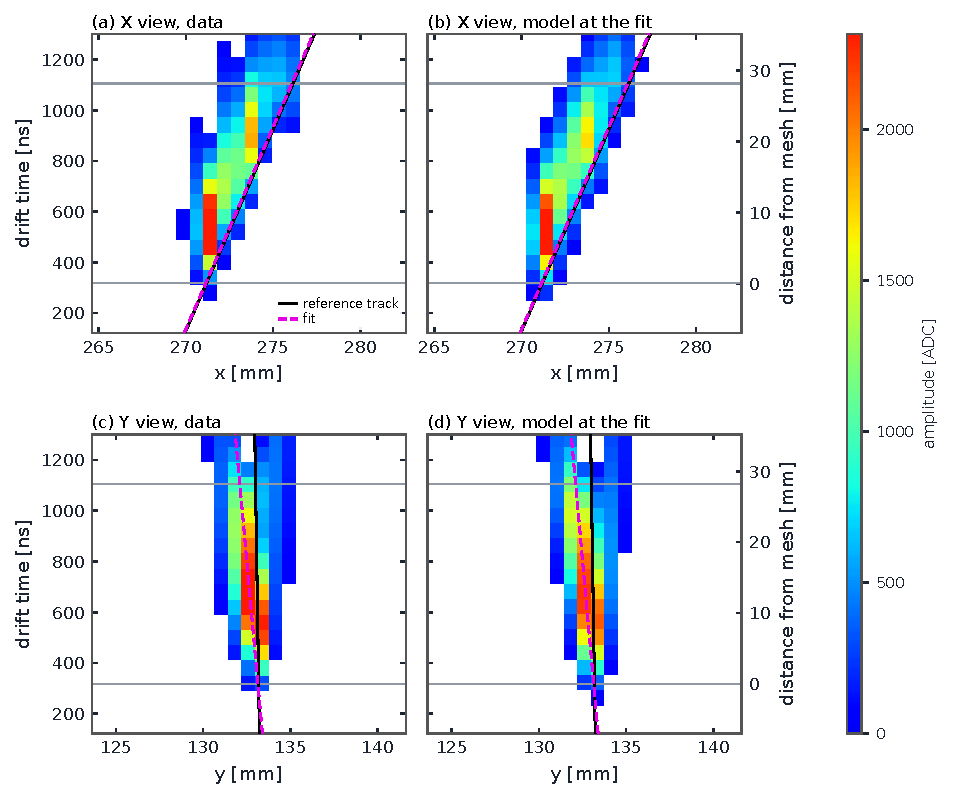
\includegraphics[width=0.74\linewidth]{muon_data_model}
  \caption{What a chamber records, and what the reconstruction fits: one cosmic muon in chamber~A (Run~1). Left, the
  data: amplitude per strip and 60\,ns sample in the X view (top) and the Y view (bottom); the track appears as a
  slanted column from the mesh ($t_0$) to the cathode ($t_0+g/\vd$, grey lines). Right, the forward model evaluated at
  the fit, on the same colour scale: the whole strip $\times$ time picture is fitted, not per-strip times. Solid black:
  the reference track; dashed: the fitted track. Each pulse lasts a few samples after its electrons arrive (the
  shaping), so the charge extends above the cathode line.}
  \label{fig:reco}
\end{figure}

\subsection{Definitions used throughout}\label{sec:definitions}
\sectionstate{partial}{new 2026-11-10: collected from the old sections 5.2, 7.6 and the caption of the angle figure, so
that each term is defined before its first use.}
\textbf{Interior.} The part of the active area at least 30\,mm from the two $x$ sides and 8\,mm from the two $y$
sides. Angles and positions are quoted in the interior, because the drift field fringes near the $x$ sides
(\cref{sec:edge}); efficiencies are quoted over the full active area unless the interior is named.
The interior is defined on the footprint of the track through the whole drift gap, in both views.
\textbf{Matched.} A reconstructed track is matched to the reference when it lies within $R=5$\,mm of the reference ray
at the mesh (\cref{sec:effdef,app:effdef}).
\textbf{$s_{68}$.} Resolutions are quoted as $s_{68}$, the 68th percentile of the absolute residual after its median
is subtracted. It equals $\sigma$ for a Gaussian and, unlike a fitted width, includes the tails.
\textbf{Voltages.} The mesh is at ground. $HV_\mathrm{resist}$, on the resistive strips, sets the gain;
$HV_\mathrm{drift}$, on the cathode, sets the drift field $E=HV_\mathrm{drift}/g$ with $g$ the measured gap
(\cref{sec:gap}).
